\documentclass[twoside]{book}

% Packages required by doxygen
\usepackage{calc}
\usepackage{doxygen}
\usepackage{graphicx}
\usepackage[utf8]{inputenc}
\usepackage{makeidx}
\usepackage{multicol}
\usepackage{multirow}
\usepackage{textcomp}
\usepackage[table]{xcolor}

% Font selection
\usepackage[T1]{fontenc}
\usepackage{mathptmx}
\usepackage[scaled=.90]{helvet}
\usepackage{courier}
\usepackage{amssymb}
\usepackage{sectsty}
\renewcommand{\familydefault}{\sfdefault}
\allsectionsfont{%
  \fontseries{bc}\selectfont%
  \color{darkgray}%
}
\renewcommand{\DoxyLabelFont}{%
  \fontseries{bc}\selectfont%
  \color{darkgray}%
}

% Page & text layout
\usepackage{geometry}
\geometry{%
  a4paper,%
  top=2.5cm,%
  bottom=2.5cm,%
  left=2.5cm,%
  right=2.5cm%
}
\tolerance=750
\hfuzz=15pt
\hbadness=750
\setlength{\emergencystretch}{15pt}
\setlength{\parindent}{0cm}
\setlength{\parskip}{0.2cm}
\makeatletter
\renewcommand{\paragraph}{%
  \@startsection{paragraph}{4}{0ex}{-1.0ex}{1.0ex}{%
    \normalfont\normalsize\bfseries\SS@parafont%
  }%
}
\renewcommand{\subparagraph}{%
  \@startsection{subparagraph}{5}{0ex}{-1.0ex}{1.0ex}{%
    \normalfont\normalsize\bfseries\SS@subparafont%
  }%
}
\makeatother

% Headers & footers
\usepackage{fancyhdr}
\pagestyle{fancyplain}
\fancyhead[LE]{\fancyplain{}{\bfseries\thepage}}
\fancyhead[CE]{\fancyplain{}{}}
\fancyhead[RE]{\fancyplain{}{\bfseries\leftmark}}
\fancyhead[LO]{\fancyplain{}{\bfseries\rightmark}}
\fancyhead[CO]{\fancyplain{}{}}
\fancyhead[RO]{\fancyplain{}{\bfseries\thepage}}
\fancyfoot[LE]{\fancyplain{}{}}
\fancyfoot[CE]{\fancyplain{}{}}
\fancyfoot[RE]{\fancyplain{}{\bfseries\scriptsize Generated on Wed Nov 22 2023 15\-:29\-:27 for C\-A\-L\-I\-B\-M\-U\-L\-T\-I by Doxygen }}
\fancyfoot[LO]{\fancyplain{}{\bfseries\scriptsize Generated on Wed Nov 22 2023 15\-:29\-:27 for C\-A\-L\-I\-B\-M\-U\-L\-T\-I by Doxygen }}
\fancyfoot[CO]{\fancyplain{}{}}
\fancyfoot[RO]{\fancyplain{}{}}
\renewcommand{\footrulewidth}{0.4pt}
\renewcommand{\chaptermark}[1]{%
  \markboth{#1}{}%
}
\renewcommand{\sectionmark}[1]{%
  \markright{\thesection\ #1}%
}

% Indices & bibliography
\usepackage{natbib}
\usepackage[titles]{tocloft}
\setcounter{tocdepth}{3}
\setcounter{secnumdepth}{5}
\makeindex

% Custom commands
\newcommand{\clearemptydoublepage}{%
  \newpage{\pagestyle{empty}\cleardoublepage}%
}


%===== C O N T E N T S =====

\begin{document}

% Titlepage & ToC
\pagenumbering{roman}
\begin{titlepage}
\vspace*{7cm}
\begin{center}%
{\Large C\-A\-L\-I\-B\-M\-U\-L\-T\-I \\[1ex]\large 1.\-1.\-0 }\\
\vspace*{1cm}
{\large Generated by Doxygen 1.8.5}\\
\vspace*{0.5cm}
{\small Wed Nov 22 2023 15:29:27}\\
\end{center}
\end{titlepage}
\clearemptydoublepage
\tableofcontents
\clearemptydoublepage
\pagenumbering{arabic}

%--- Begin generated contents ---
\chapter{Hierarchical Index}
\section{Class Hierarchy}
This inheritance list is sorted roughly, but not completely, alphabetically\-:\begin{DoxyCompactList}
\item I\-Conditions\-Change\-Listener\begin{DoxyCompactList}
\item \contentsline{section}{C\-A\-L\-I\-C\-E\-:\-:multi\-Calibrator}{\pageref{classCALICE_1_1multiCalibrator}}{}
\end{DoxyCompactList}
\item Processor\begin{DoxyCompactList}
\item \contentsline{section}{C\-A\-L\-I\-C\-E\-:\-:multi\-Calibrator}{\pageref{classCALICE_1_1multiCalibrator}}{}
\end{DoxyCompactList}
\item T\-Object\begin{DoxyCompactList}
\item \contentsline{section}{T\-Convolution}{\pageref{classTConvolution}}{}
\end{DoxyCompactList}
\end{DoxyCompactList}

\chapter{Class Index}
\section{Class List}
Here are the classes, structs, unions and interfaces with brief descriptions\-:\begin{DoxyCompactList}
\item\contentsline{section}{{\bf C\-A\-L\-I\-C\-E\-::multi\-Calibrator} \\*Processor to add P\-A\-R\-\_\-\-M\-U\-L\-T\-I to the event and calibrate the threshold }{\pageref{classCALICE_1_1multiCalibrator}}{}
\item\contentsline{section}{{\bf T\-Convolution} \\*R\-O\-O\-T class which generates the convolution of two functions }{\pageref{classTConvolution}}{}
\end{DoxyCompactList}

\chapter{Class Documentation}
\section{C\-A\-L\-I\-C\-E\-:\-:multi\-Calibrator Class Reference}
\label{classCALICE_1_1multiCalibrator}\index{C\-A\-L\-I\-C\-E\-::multi\-Calibrator@{C\-A\-L\-I\-C\-E\-::multi\-Calibrator}}


Processor to add P\-A\-R\-\_\-\-M\-U\-L\-T\-I to the event and calibrate the threshold.  




{\ttfamily \#include $<$multi\-Calibrator.\-hh$>$}

Inheritance diagram for C\-A\-L\-I\-C\-E\-:\-:multi\-Calibrator\-:\begin{figure}[H]
\begin{center}
\leavevmode
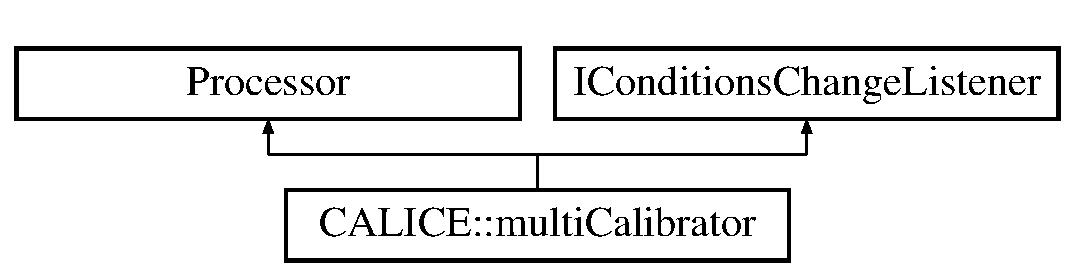
\includegraphics[height=2.000000cm]{classCALICE_1_1multiCalibrator}
\end{center}
\end{figure}
\subsection*{Public Member Functions}
\begin{DoxyCompactItemize}
\item 
Processor $\ast$ {\bfseries new\-Processor} ()\label{classCALICE_1_1multiCalibrator_ad18beb97b5deccfa062ed368644fce16}

\item 
virtual void {\bfseries init} ()\label{classCALICE_1_1multiCalibrator_a8a3e419d429f42b6ea7aae4b52428ce4}

\item 
virtual void {\bfseries process\-Run\-Header} (L\-C\-Run\-Header $\ast$run)\label{classCALICE_1_1multiCalibrator_a67d14b42a9ce88fc17515613efe997bc}

\item 
virtual void {\bfseries process\-Event} (L\-C\-Event $\ast$evt)\label{classCALICE_1_1multiCalibrator_a7664b108349a27d1497d52d55001dc41}

\item 
virtual void {\bfseries end} ()\label{classCALICE_1_1multiCalibrator_a156e6823b5819c32c0c1530f9cf17787}

\item 
virtual void {\bfseries conditions\-Changed} (lcio\-::\-L\-C\-Collection $\ast$col)\label{classCALICE_1_1multiCalibrator_aae74a036fde33453359d9938bacd8475}

\end{DoxyCompactItemize}
\subsection*{Protected Attributes}
\begin{DoxyCompactItemize}
\item 
std\-::string {\bfseries \-\_\-adc\-Col\-Name}\label{classCALICE_1_1multiCalibrator_a2c6dadc7bd856f48ebabb2ff1f3eb24d}

\item 
std\-::string {\bfseries \-\_\-par\-Name\-Trigger\-Event}\label{classCALICE_1_1multiCalibrator_a9dcf1a278390cf22a27f873b03ecaf42}

\item 
std\-::string {\bfseries \-\_\-output\-File\-Path}\label{classCALICE_1_1multiCalibrator_a243d6d66340eba9a2cadfa2387b20c0f}

\item 
std\-::string {\bfseries \-\_\-connection\-Col\-Name}\label{classCALICE_1_1multiCalibrator_acd73797da60310a0a4bcfd495204a855}

\item 
std\-::string {\bfseries \-\_\-reference\-Threshold\-Col\-Name}\label{classCALICE_1_1multiCalibrator_ac3f8d6ece5b4b56d26a9864ee0618ce5}

\item 
std\-::string {\bfseries \-\_\-skip\-Calibration}\label{classCALICE_1_1multiCalibrator_af3bb02c62940673fb59d5250cc294d6d}

\item 
Float\-Vec {\bfseries \-\_\-signal\-Binning}\label{classCALICE_1_1multiCalibrator_aa88fe075d6603ee3c78158bd742b91e4}

\item 
Float\-Vec {\bfseries \-\_\-purity\-List}\label{classCALICE_1_1multiCalibrator_a8d8b4bb7da03c22ddf35a8f94c7bb1a0}

\item 
float {\bfseries \-\_\-gaus\-Range}\label{classCALICE_1_1multiCalibrator_a7fc0a223ac7ef8119b3b0a987eb44adc}

\item 
int {\bfseries \-\_\-rebin}\label{classCALICE_1_1multiCalibrator_a007fb7a565ad1ec0eb2719981203f8fe}

\item 
int {\bfseries \-\_\-gran\-Fac}\label{classCALICE_1_1multiCalibrator_a5dcaedfa4e29bad191bc22016eca0355}

\end{DoxyCompactItemize}
\subsection*{Private Types}
\begin{DoxyCompactItemize}
\item 
typedef std\-::map$<$ float, float $>$ {\bfseries Threshold\-Map\-\_\-t}\label{classCALICE_1_1multiCalibrator_a35b415a32f3bf4f78a4bb5adc3f96470}

\end{DoxyCompactItemize}
\subsection*{Private Member Functions}
\begin{DoxyCompactItemize}
\item 
void {\bfseries fill\-Hist} (T\-H1\-F $\ast$hist, L\-C\-Event $\ast$evt)\label{classCALICE_1_1multiCalibrator_a0f54d7d5a1e9b4469bc59ae7b2d3a204}

\end{DoxyCompactItemize}
\subsection*{Private Attributes}
\begin{DoxyCompactItemize}
\item 
lccd\-::\-L\-C\-C\-D\-Time\-Stamp {\bfseries \-\_\-start\-Time}\label{classCALICE_1_1multiCalibrator_a33b407cfd46e3ac56bdc30947e0eb2e1}

\item 
lccd\-::\-L\-C\-C\-D\-Time\-Stamp {\bfseries \-\_\-end\-Time}\label{classCALICE_1_1multiCalibrator_a06d7b62ae49be9bad5c7eb8a7f270f58}

\item 
unsigned {\bfseries \-\_\-run\-Number}\label{classCALICE_1_1multiCalibrator_acfcabcaf4253473ac3d99df1f162da5f}

\item 
unsigned int {\bfseries \-\_\-crate}\label{classCALICE_1_1multiCalibrator_afc05f707dab2f811d755300d480d57f6}

\item 
unsigned int {\bfseries \-\_\-slot}\label{classCALICE_1_1multiCalibrator_a88106b2a17b0308851dfdace4d9fd8a4}

\item 
unsigned int {\bfseries \-\_\-fe}\label{classCALICE_1_1multiCalibrator_a7e31fc8c645ee72b61deafacb51ee6b5}

\item 
unsigned int {\bfseries \-\_\-chip}\label{classCALICE_1_1multiCalibrator_ae8423d1b22561196f45134990b6e3be5}

\item 
unsigned int {\bfseries \-\_\-channel}\label{classCALICE_1_1multiCalibrator_a1a14cc1103c22d000ea6565619bc98ee}

\item 
T\-H1\-F $\ast$ {\bfseries \-\_\-sig\-Hist}\label{classCALICE_1_1multiCalibrator_a5087ce6fdd939090347791bc86a02025}

\item 
T\-H1\-F $\ast$ {\bfseries \-\_\-ped\-Hist}\label{classCALICE_1_1multiCalibrator_abf5102e26fbe03d997813b06eea13818}

\item 
bool {\bfseries \-\_\-connection\-Available}\label{classCALICE_1_1multiCalibrator_adcb7ef44a6a00a92da355ee43dbcc147}

\item 
Threshold\-Map\-\_\-t {\bfseries \-\_\-reference\-Thresholds}\label{classCALICE_1_1multiCalibrator_ac2eccfcf6a4b10389fabf83c743a9b0d}

\end{DoxyCompactItemize}


\subsection{Detailed Description}
Processor to add P\-A\-R\-\_\-\-M\-U\-L\-T\-I to the event and calibrate the threshold. 

This processor adds an event parameter containing the amplitude of the analog multiplicity counter readout. In addition a histogram of the amplitudes is collected and fitted to calibrate the multi threshold. The calibration procedure can be skipped by processor parameter. In this case, only the event parameter is added.

The mapping of the multiplicity counter connection is read from the L\-C\-I\-O stream.

The results of the calibration can be written directly to a L\-C\-C\-D database. To enable this feature, M\-U\-L\-T\-I\-\_\-\-D\-B\-I\-N\-I\-T has to contain a valid database connection string for write access at compile time. In this case, two processor parameters to set the output folders for thresholds and fraction of rejected events are available. If the string for a folder is empty, the writing of this folder will be skipped.

\begin{DoxyVersion}{Version}
1.\-0 
\end{DoxyVersion}
\begin{DoxyAuthor}{Author}
{\tt Benjamin.\-Lutz@desy.\-de} 
\end{DoxyAuthor}
\begin{DoxyDate}{Date}
Sep 2008 
\end{DoxyDate}


Definition at line 36 of file multi\-Calibrator.\-hh.



The documentation for this class was generated from the following files\-:\begin{DoxyCompactItemize}
\item 
/nfs/dust/ilc/user/marquezh/\-Calice\-Soft\-\_\-w\-\_\-\-I\-L\-C\-Soft\-\_\-v02-\/03-\/02/calice\-\_\-calib/calibmulti/include/multi\-Calibrator.\-hh\item 
/nfs/dust/ilc/user/marquezh/\-Calice\-Soft\-\_\-w\-\_\-\-I\-L\-C\-Soft\-\_\-v02-\/03-\/02/calice\-\_\-calib/calibmulti/src/multi\-Calibrator.\-cc\end{DoxyCompactItemize}

\section{T\-Convolution Class Reference}
\label{classTConvolution}\index{T\-Convolution@{T\-Convolution}}


R\-O\-O\-T class which generates the convolution of two functions.  




{\ttfamily \#include $<$T\-Convolution.\-h$>$}

Inheritance diagram for T\-Convolution\-:\begin{figure}[H]
\begin{center}
\leavevmode
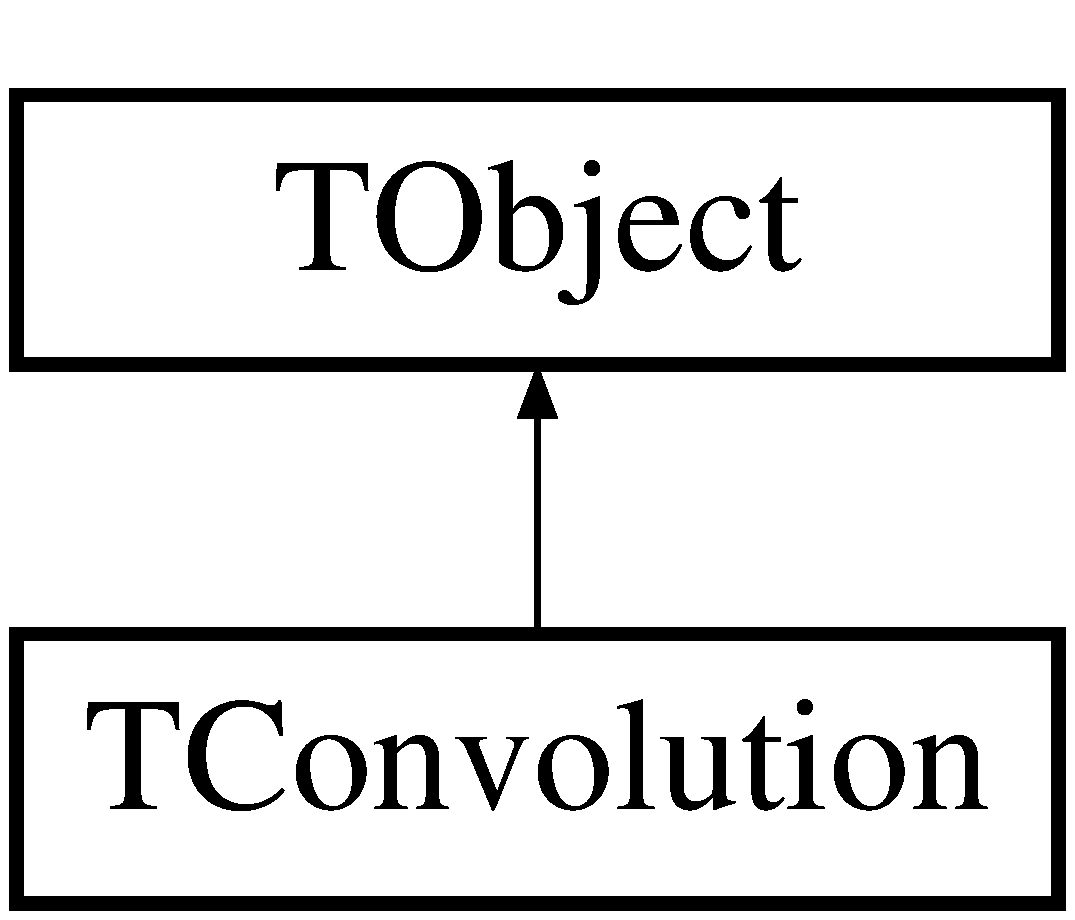
\includegraphics[height=2.000000cm]{classTConvolution}
\end{center}
\end{figure}
\subsection*{Public Member Functions}
\begin{DoxyCompactItemize}
\item 
{\bf T\-Convolution} ()\label{classTConvolution_a5efa34bb8cd60e092581b64224ed8410}

\begin{DoxyCompactList}\small\item\em Standard constructor. The \doxyref{Init()}{p.}{classTConvolution_a432fc14c48910df995d2a7fe6c6a1573} function has to be used to set the parameters. \end{DoxyCompactList}\item 
{\bf T\-Convolution} (const char $\ast$name, T\-F1 $\ast$f1, T\-F1 $\ast$f2, bool add\-Scale=true, Int\-\_\-t steps\-Per\-Point=50)\label{classTConvolution_a158f63a9c229919ffe33c2dd5feadcd7}

\begin{DoxyCompactList}\small\item\em Constructor with initialisation parameters. See \doxyref{Init()}{p.}{classTConvolution_a432fc14c48910df995d2a7fe6c6a1573} function for parameter description. \end{DoxyCompactList}\item 
void {\bf Init} (const char $\ast$name, T\-F1 $\ast$f1, T\-F1 $\ast$f2, bool add\-Scale=true, Int\-\_\-t steps\-Per\-Point=50)
\begin{DoxyCompactList}\small\item\em Initialisation function. \end{DoxyCompactList}\item 
T\-F1 $\ast$ {\bf Get\-Convoluted\-Function} ()
\begin{DoxyCompactList}\small\item\em get the resulting function \end{DoxyCompactList}\item 
T\-F1 $\ast$ {\bf Get\-F1} ()
\begin{DoxyCompactList}\small\item\em get access to the first internal function \end{DoxyCompactList}\item 
T\-F1 $\ast$ {\bf Get\-F2} ()
\begin{DoxyCompactList}\small\item\em get access to the second internal function \end{DoxyCompactList}\item 
Double\-\_\-t {\bf operator()} (Double\-\_\-t $\ast$x, Double\-\_\-t $\ast$par)
\end{DoxyCompactItemize}
\subsection*{Private Member Functions}
\begin{DoxyCompactItemize}
\item 
Double\-\_\-t {\bfseries integrand} (Double\-\_\-t t, Double\-\_\-t x0)\label{classTConvolution_a0dc90fb152886b2fa811f065c0775bc8}

\item 
Double\-\_\-t {\bfseries convolution\-Fkt} (Double\-\_\-t $\ast$x, Double\-\_\-t $\ast$par)\label{classTConvolution_ae040a18550d990845ea41546b88560ae}

\end{DoxyCompactItemize}
\subsection*{Private Attributes}
\begin{DoxyCompactItemize}
\item 
std\-::string {\bfseries \-\_\-name}\label{classTConvolution_aae8d0e128e4bb487012cb1ef752c43be}

\item 
T\-F1 $\ast$ {\bfseries \-\_\-f1}\label{classTConvolution_a00ebb43017df7488e21e927e18162c1f}

\item 
T\-F1 $\ast$ {\bfseries \-\_\-f2}\label{classTConvolution_adea7f44d58c4d909e0b75d41157344c2}

\item 
T\-F1 $\ast$ {\bfseries \-\_\-convolution}\label{classTConvolution_ac9a1f348cabcb8b0ed86992c279586ce}

\item 
Int\-\_\-t {\bfseries \-\_\-n\-Par1}\label{classTConvolution_a06390a21505766c7fd74debd2c15dde7}

\item 
Int\-\_\-t {\bfseries \-\_\-n\-Par2}\label{classTConvolution_a31ba676b4d6b87c003f32cfc77e9a47a}

\item 
Int\-\_\-t {\bfseries \-\_\-base\-Npar}\label{classTConvolution_a706f57e007e699039dd4b5086b4dd554}

\item 
Int\-\_\-t {\bfseries \-\_\-steps\-Per\-Point}\label{classTConvolution_a2e1a7d63609f597d36687951a65d3f76}

\item 
Int\-\_\-t {\bfseries \-\_\-scale\-Par\-Number}\label{classTConvolution_a9d789055255d62e4382a10ea4a737f07}

\item 
Double\-\_\-t {\bfseries \-\_\-f1\-Rmin}\label{classTConvolution_a1d4d04a8a3a18837ad56a0c195dbd1fe}

\item 
Double\-\_\-t {\bfseries \-\_\-f1\-Rmax}\label{classTConvolution_a642c24cf3216b284609800223e082f39}

\item 
Double\-\_\-t {\bfseries \-\_\-f2\-Rmin}\label{classTConvolution_a351a86c5c23a95c553f47e09769ba12f}

\item 
Double\-\_\-t {\bfseries \-\_\-f2\-Rmax}\label{classTConvolution_a7b5a24abf8305bd1080c7ee5ed037153}

\item 
Double\-\_\-t {\bfseries \-\_\-\-Rmin}\label{classTConvolution_a642dd1c40e701d0b41188b4e1bcc6e4b}

\item 
Double\-\_\-t {\bfseries \-\_\-\-Rmax}\label{classTConvolution_aab18051f17a5697a23e908feee026195}

\item 
bool {\bfseries \-\_\-add\-Scale}\label{classTConvolution_afccab6bf0322cc5a07b014c30f52367e}

\end{DoxyCompactItemize}


\subsection{Detailed Description}
R\-O\-O\-T class which generates the convolution of two functions. 

The convoluted function corresponds to \[ f_{conv}(x) = \int_{min_{i}}^{max_{i}}{f_{1}(t) \cdot f_{2}(x-t) \textrm{d}t} \] where $ min_{i} $ ( $ max_{i} $) is the minimum (maximum) of the range of function $ f_{i} $. The integral is calculated as the Riemann sum with selectable number of steps.

The range of the input function $ f_{1} $ and the number of steps in the integration have to be chosen reasonably to achieve a good result with a acceptable computing effort. If the integral of one of the functions is easier to approximate it should be used as $ f_{1} $.

An additional scaling parameter can be muliplied to the result of the convolution. This is for fitting to data.

\begin{DoxyAttention}{Attention}
This class needs R\-O\-O\-T version 5.\-16 or above.
\end{DoxyAttention}
\begin{DoxyAuthor}{Author}
{\tt Benjamin.\-Lutz@desy.\-de} 
\end{DoxyAuthor}
\begin{DoxyVersion}{Version}
1.\-0 
\end{DoxyVersion}
\begin{DoxyDate}{Date}
September 2008 
\end{DoxyDate}


Definition at line 31 of file T\-Convolution.\-h.



\subsection{Member Function Documentation}
\index{T\-Convolution@{T\-Convolution}!Get\-Convoluted\-Function@{Get\-Convoluted\-Function}}
\index{Get\-Convoluted\-Function@{Get\-Convoluted\-Function}!TConvolution@{T\-Convolution}}
\subsubsection[{Get\-Convoluted\-Function}]{\setlength{\rightskip}{0pt plus 5cm}T\-F1 $\ast$ T\-Convolution\-::\-Get\-Convoluted\-Function (
\begin{DoxyParamCaption}
{}
\end{DoxyParamCaption}
)}\label{classTConvolution_a4f2e261e138ae00dd6eec73fbfd57cdc}


get the resulting function 

\begin{DoxyReturn}{Returns}
pointer to the convoluted function 
\end{DoxyReturn}


Definition at line 43 of file T\-Convolution.\-cc.

\index{T\-Convolution@{T\-Convolution}!Get\-F1@{Get\-F1}}
\index{Get\-F1@{Get\-F1}!TConvolution@{T\-Convolution}}
\subsubsection[{Get\-F1}]{\setlength{\rightskip}{0pt plus 5cm}T\-F1$\ast$ T\-Convolution\-::\-Get\-F1 (
\begin{DoxyParamCaption}
{}
\end{DoxyParamCaption}
)\hspace{0.3cm}{\ttfamily [inline]}}\label{classTConvolution_a57a972c335a8c28fdd2c8ff348544935}


get access to the first internal function 

\begin{DoxyReturn}{Returns}
pointer to the internal copy of the first function 
\end{DoxyReturn}


Definition at line 68 of file T\-Convolution.\-h.

\index{T\-Convolution@{T\-Convolution}!Get\-F2@{Get\-F2}}
\index{Get\-F2@{Get\-F2}!TConvolution@{T\-Convolution}}
\subsubsection[{Get\-F2}]{\setlength{\rightskip}{0pt plus 5cm}T\-F1$\ast$ T\-Convolution\-::\-Get\-F2 (
\begin{DoxyParamCaption}
{}
\end{DoxyParamCaption}
)\hspace{0.3cm}{\ttfamily [inline]}}\label{classTConvolution_a8abb64b348b2d26d5cf245984858b144}


get access to the second internal function 

\begin{DoxyReturn}{Returns}
pointer to the second copy of the first function 
\end{DoxyReturn}


Definition at line 73 of file T\-Convolution.\-h.

\index{T\-Convolution@{T\-Convolution}!Init@{Init}}
\index{Init@{Init}!TConvolution@{T\-Convolution}}
\subsubsection[{Init}]{\setlength{\rightskip}{0pt plus 5cm}void T\-Convolution\-::\-Init (
\begin{DoxyParamCaption}
\item[{const char $\ast$}]{name, }
\item[{T\-F1 $\ast$}]{f1, }
\item[{T\-F1 $\ast$}]{f2, }
\item[{bool}]{add\-Scale = {\ttfamily true}, }
\item[{Int\-\_\-t}]{steps\-Per\-Point = {\ttfamily 50}}
\end{DoxyParamCaption}
)}\label{classTConvolution_a432fc14c48910df995d2a7fe6c6a1573}


Initialisation function. 


\begin{DoxyParams}{Parameters}
{\em name} & Name of the resulting convoluted function. This is the R\-O\-O\-T-\/\-Object-\/name and has to be unique. \\
\hline
{\em f1} & First function of the convolution \\
\hline
{\em f2} & Second function of the convolution \\
\hline
{\em add\-Scale} & If this is true, a scale parameter is multiplied to the result of the convolution. This allows to use normalized functions in the convolution. The R\-O\-O\-T T\-F1-\/parameter number will be $ N_{f1} + N_{f2} + 1 $, where $ N_{x} $ is the number of parameters of input funciton $ x $ \\
\hline
{\em steps\-Per\-Point} & Number of steps in the approximation of the convolution integral. \\
\hline
\end{DoxyParams}


Definition at line 19 of file T\-Convolution.\-cc.



Referenced by T\-Convolution().

\index{T\-Convolution@{T\-Convolution}!operator()@{operator()}}
\index{operator()@{operator()}!TConvolution@{T\-Convolution}}
\subsubsection[{operator()}]{\setlength{\rightskip}{0pt plus 5cm}Double\-\_\-t T\-Convolution\-::operator() (
\begin{DoxyParamCaption}
\item[{Double\-\_\-t $\ast$}]{x, }
\item[{Double\-\_\-t $\ast$}]{par}
\end{DoxyParamCaption}
)\hspace{0.3cm}{\ttfamily [inline]}}\label{classTConvolution_a35cbc0ef409d8128c0ad1363b90f9dc5}
This operator allows that the class can be used to initialise a R\-O\-O\-T T\-F1() function


\begin{DoxyParams}{Parameters}
{\em x} & pointer to array of input variables (in this case pointer to x) \\
\hline
{\em par} & pointer to array of function parameters \\
\hline
\end{DoxyParams}
\begin{DoxyReturn}{Returns}
value of the convoluted function 
\end{DoxyReturn}


Definition at line 82 of file T\-Convolution.\-h.



The documentation for this class was generated from the following files\-:\begin{DoxyCompactItemize}
\item 
/nfs/dust/ilc/user/marquezh/\-Calice\-Soft\-\_\-w\-\_\-\-I\-L\-C\-Soft\-\_\-v02-\/03-\/02/calice\-\_\-calib/calibmulti/include/T\-Convolution.\-h\item 
/nfs/dust/ilc/user/marquezh/\-Calice\-Soft\-\_\-w\-\_\-\-I\-L\-C\-Soft\-\_\-v02-\/03-\/02/calice\-\_\-calib/calibmulti/src/T\-Convolution.\-cc\end{DoxyCompactItemize}

%--- End generated contents ---

% Index
\newpage
\phantomsection
\addcontentsline{toc}{part}{Index}
\printindex

\end{document}
